\documentclass[a4paper,11pt]{article}

\usepackage{préambule}
\usetikzlibrary{matrix,arrows,positioning}

\begin{document}

\begin{methode}
	Pour trouver une quatrième proportionnelle :
	\begin{itemize}
		\item Une des colonnes du tableau est remplie : on peut donc trouver le \\ \uline{coefficient de proportionnalité}.
		\item Si la valeur manquante est en bas, on \textbf{multiplie} la case au dessus par le coefficient de proportionnalité.
		\item Si la valeur manquante est en haut, on \textbf{divise} la case en dessous par le coefficient de proportionnalité.
	\end{itemize}
\end{methode}

\begin{exemple}
	On sait que le tableau suivant est proportionnel :

	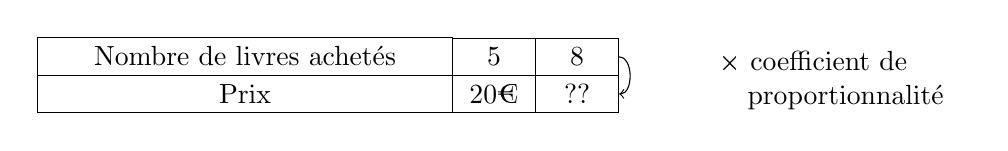
\begin{tikzpicture}
		\matrix (tableau) [
			nodes={rectangle,draw=black,minimum width=3em},
			matrix of nodes,
			row sep=-\pgflinewidth,
			column sep=-\pgflinewidth,
			column 1/.style={
					minimum width=15em,
					nodes={rectangle,draw=black,minimum width=15em}
				}]{
			Nombre de livres achetés & 5   & 8  \\
			Prix                     & 20€ & ?? \\
		};
		\draw[->] (tableau-1-3.east) to [out=0,in=0] (tableau-2-3.east);
		\node[text width=4cm,align=center] at ([xshift=3cm,yshift=-0.3cm] tableau-1-3) {× coefficient de\\ \hspace{2em} proportionnalité};
	\end{tikzpicture}  \\
	Le coefficient de proportionnalité est
	$$ 20 ÷ 5 = 4 $$
	Donc le prix de 8 livres est
	$$ 8 × 4 = 32€ $$
\end{exemple}

\vspace{3em}
\hrule
\vspace{2em}

\begin{methode}
	Pour trouver une quatrième proportionnelle :
	\begin{itemize}
		\item Une des colonnes du tableau est remplie : on peut donc trouver le \\ \uline{coefficient de proportionnalité}.
		\item Si la valeur manquante est en bas, on \textbf{multiplie} la case au dessus par le coefficient de proportionnalité.
		\item Si la valeur manquante est en haut, on \textbf{divise} la case en dessous par le coefficient de proportionnalité.
	\end{itemize}
\end{methode}

\begin{exemple}
	On sait que le tableau suivant est proportionnel :

	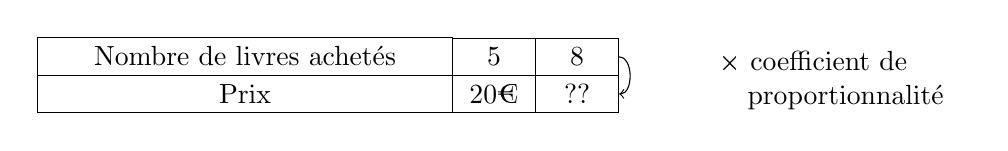
\begin{tikzpicture}
		\matrix (tableau) [
			nodes={rectangle,draw=black,minimum width=3em},
			matrix of nodes,
			row sep=-\pgflinewidth,
			column sep=-\pgflinewidth,
			column 1/.style={
					minimum width=15em,
					nodes={rectangle,draw=black,minimum width=15em}
				}]{
			Nombre de livres achetés & 5   & 8  \\
			Prix                     & 20€ & ?? \\
		};
		\draw[->] (tableau-1-3.east) to [out=0,in=0] (tableau-2-3.east);
		\node[text width=4cm,align=center] at ([xshift=3cm,yshift=-0.3cm] tableau-1-3) {× coefficient de\\ \hspace{2em} proportionnalité};
	\end{tikzpicture} \\
	Le coefficient de proportionnalité est
	$$ 20 ÷ 5 = 4 $$
	Donc le prix de 8 livres est
	$$ 8 × 4 = 32€ $$
\end{exemple}

\end{document}